% 导数
% 微积分|导数|导函数|切线|极限

% 未完成: 举几个例子,说明常数导数为零, 直线导数为定值等!
\pentry{极限\upref{Lim}}

\subsection{导数的几何理解}

一个一元函数 $y = f(x)$, 在直角坐标系中表示为一条曲线.在这个曲线的光滑部分取一点 $A$, 并作其切线\upref{TanL}.

\begin{figure}[ht]
\centering
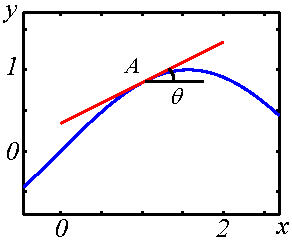
\includegraphics[width=5cm]{./figures/Der1.pdf}
\caption{点 $A$ 的切线}
\end{figure}


若切线存在,该切线与 $x$ 轴的夹角 的正切值 $\theta$ 就叫点 $A$ 的导数.当函数在 $A$ 点递增时,可能的取值为 $\theta \in (0,\pi/2)$, 即 $\tan \theta  \in (0, + \infty)$. 递减时,取 $\theta  \in (-\pi/2,0)$, 即 $\tan \theta \in (-\infty ,0)$. 当切线水平时,$\theta  = \tan \theta  = 0$. 

若函数曲线在 $x$ 的某一开区间内的每一点都可导, 则这个区间上每一个 $x$ 对应一个导数.将其写成关于 $x$ 的函数 $g(x)$,  $g(x)$  就是该区间上的 \textbf{导函数}. 通常将导函数记为以下的一种(后3种记号的来源见下文)

\begin{equation}\label{Der_eq1}
f'(x),\quad [f(x)]',\quad \dv{y}{x},\quad \dv{f}{x},\quad \dv{x}f(x)
\end{equation}
在物理中, 常常在物理量上方加一点表示对时间求导(注意仅限于对时间求导), 例如 $\dot f(t) = \dv*{f(t)}{t}$.

若切线不存在(例如折线的棱角处,但也有其他更复杂的情况), 我们说点 $A$ 不可导.

\begin{figure}[ht]
\centering
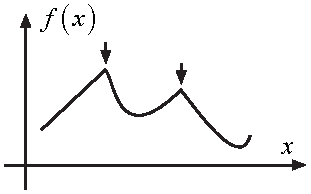
\includegraphics[width=5cm]{./figures/Der3.pdf}
\caption{棱角处不可导}
\end{figure}

若函数曲线在某一点附近是光滑的,那么在这点附近取一小段,当这一段取得足够小,可以近似认为它是线段且与切线重合(如下图). 以这条线段为斜边,作一直角三角形,令其底边长为 $\dd{x}$ (在微积分中,通常把非常小的一段 $\Delta x$ 记为 $\dd{x}$,  $\dd{x}$ 是一不能分割的整体符号,而不是两个量相乘),竖直边的边长为 $\dd{y}$ (当函数递增时, $\dd{y}$ 取正值,反之取负值).根据上面导数的定义,$\dv*{y}{x} = \tan \theta $ 就是函数的导数.所以导数通常表示为 $\dv*{y}{x}$, 导数的倒数则为 $\dv*{x}{y}$. 

\begin{figure}[ht]
\centering
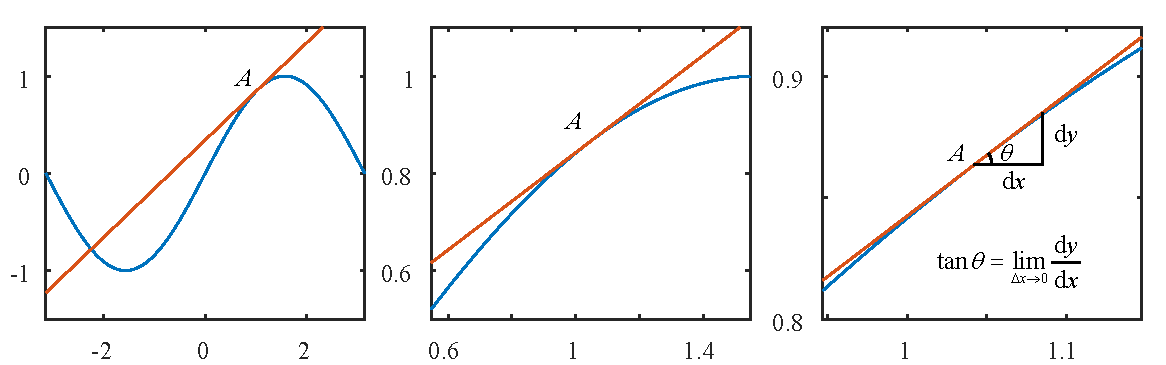
\includegraphics[width=14cm]{./figures/Der2.pdf}
\caption{将切点放大,会发现切线和曲线在切点附近“重合”}
\end{figure}

由上面的讨论可得,当 $x$ 增加一小段 $\Delta x$ 时,$y$ 轴的增量约为 $\Delta y \approx f'(x)\Delta x$,且当 $\Delta x$ 越小,这条式子就越精确成立, 记为 $\dd{y} = f'(x) \dd{x}$.这个关系就叫函数的微分.

\subsection{导数的代数理解}
导数的代数理解就是: 一个量关于另一个量的变化率. 例如质点直线运动时,速度的大小就是其路程对时间的导数.把这种描述用极限\upref{Lim}表达出来就是
\begin{equation}\label{Der_eq2}
f'(x) = \lim_{\Delta x \to 0} \frac{f(x + \Delta x) - f(x)}{\Delta x}
\end{equation}
在图3的右图中,$\Delta x$ 的始末位置并不非常重要,既可以从 $x$ 取到 $x + \Delta x$, 也可以从 $x - \Delta x$  取到 $x$ 等等( 因为当 $\Delta x$ 非常小的时候,$x$ 附近的曲线基本处处跟切线重合,它们的斜率都是一样的). 所以导数的定义也有其他类似的形式

\begin{equation}
f'(x) = \lim_{\Delta x \to 0} \frac{f(x) - f(x - \Delta x)}{\Delta x} = \lim_{\Delta x \to 0} \frac{f(x + \Delta x) - f(x - \Delta x)}{2\Delta x}
\end{equation}
虽然上面用到了诸如“近似”等词,但根据定义,极限都是精确的.

\eentry{一维运动的速度定义,一维运动的加速度定义}
